\chapter{後端架構}
\section{技術介紹}
首先使用超解析化神經網路技術將超低解析度照片做高解析化,再利 用Darknet平台所編寫特殊設計的CNN抓取手部位置。將抓取的機率分布,再使用LSTM神經網路辨識手勢,通過函數轉換與計算後,回傳發射參數(速度)。

由於server必須要確保每秒傳輸照片數,所以傳輸至後端的畫質非常低,導致偵測的準確度較低。所以首先需要克服低解析度問題,讓準確度變高。
為了讓使用者有良好的遊戲體驗,在使用者在射飛鏢時,需要馬上就能得到回應,並將飛鏢發射出去。因此需要壓縮CNN,讓計算上能更加流暢,使回傳速度更快(response time降低)。除此之外,原本darknet設計是需要將收到的照片寫入硬碟再讀取,速度極慢,需要修改內程式使darknet可以直接寫入記憶體,並直接偵測,回傳結果。


\section{技術說明與實作}


\begin{table}[]
\begin{tabular}{|l|l|l|l|l|}
\hline
    & 訓練環境                 & 伺服器環境                        \\\hline
GPU & RTX2070                  & GTX1080ti                                     \\\hline
CPU & Intel Core (TM) i7-8750H & Intel(R) Xeon(R) CPU E5-2620 v4  2.10@GHz     \\\hline
RAM & 16GB                     & 264GB                                   
\\\hline
\end{tabular}
\end{table}


\subsection{後端神經網路系統架構圖}

主要分為四部份,分別為SRCNN、手部物件辨識、LSTM以及特殊函數轉換。首先利用SRCNN將手機傳來的照片做高解析化,使手部物件辨識模型辨識率提高。在將手部辨識結果的機率分布傳至LSTM做發射手勢辨識。最後通過函數轉換後回傳發射參數,流程圖請見Figure 3.1。

\begin{figure}[H]
    \centering
    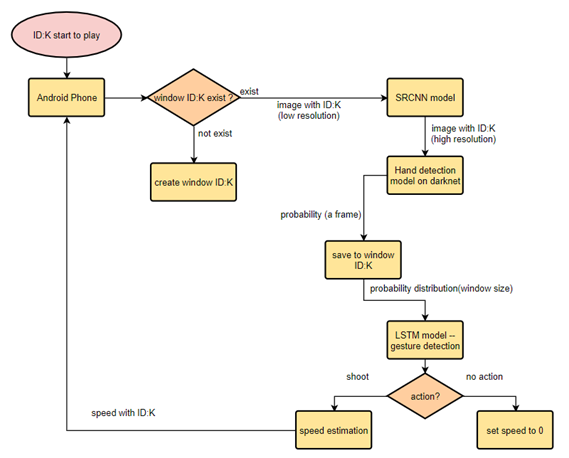
\includegraphics[width=10cm]{NN_SYS_structure.png}
    \caption{後端辨識系統架構圖}
    \label{fig:後端辨識系統架構圖}
\end{figure}

\subsubsection{SRCNN網路結構}
此處利用CNN神經網路將低解析度轉換為高解析度,以符合本地端訓練的照片高解析風格。以下呈現整體架構圖。

\begin{figure}[H]
    \centering
    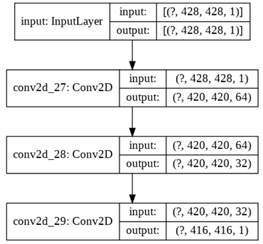
\includegraphics[width=6cm]{SRCNN_Structrue.png}
    \caption{SRCNN網路架構圖}
    \label{fig:SRCNN網路架構圖}
\end{figure}
\subsubsection{手部物件神經網路}

此專案是飛鏢遊戲,所以運算時間以及讀取時間需要降低,讓使用者不須等待就能得到射擊結果。
透過darknet平台,以yolov3為基礎更改其網路架構,以達成專屬類別輸出以及減少浮點運算次數的效果。並且,修改內部程式,達到傳輸效能提升,減少讀取時間。以下呈現經過多次實驗得到的新型網路架構。
\begin{figure}[H]
    \centering
    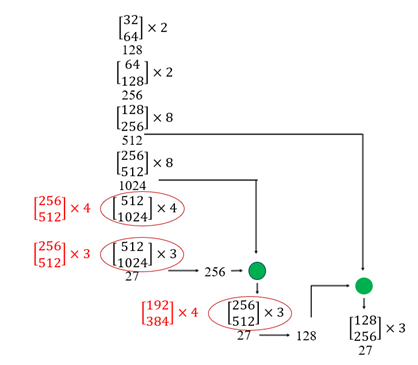
\includegraphics[width=8cm]{Darknet_Network.png}
    \caption{手部辨識神經網路架構圖(加速版)}
    \label{fig:手部辨識神經網路架構圖(加速版)}
\end{figure}



\subsubsection{LSTM神經網路}
手部物件辨識的機率分布存入window輸入至專門架設的LSTM網路結構中,並將輸出部份分為兩類別:無動作(0)、 射擊(1)。由於訓練資料的複雜度經過實驗後,發現並不需要使用更複雜的網路架構做學習,所以最終設計單層的LSTM。以下呈現LSTM網路架構。

\begin{figure}[H]
    \centering
    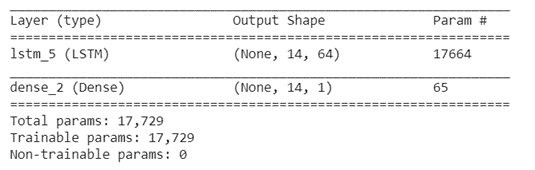
\includegraphics[width=8cm]{LSTM_Network.png}
    \caption{LSTM神經網路架構}
    \label{fig:LSTM神經網路架構}
\end{figure}


\subsection{神經網路實驗}

\subsubsection{優化darknet輸入評估實驗}

目的: 測試經過優化輸入後的darknet 與未優化輸入的darknet整體運作效能差距。
說明: 修改darknet中底層程式,並修改makefile後,重新編譯。讓darknet能加載numpy的內容,以及可以輸入陣列給darknet做偵測。而不需要再從硬碟讀取圖片作為輸入。
實驗方法:
\begin{itemize}
\item 實驗一未優化darknet輸入至原Yolo神經網路(未壓縮)做偵測。
\item 實驗二優化darknet輸入至原Yolo神經網路(未壓縮)做偵測。
\end{itemize}

測試方法:測試照片共100張的總時間,取平均時間。
\begin{figure}[H]
    \centering
    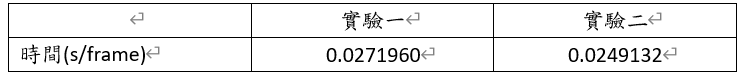
\includegraphics[width=10cm]{Darknet_Physics_Layer_OP.PNG}
    \caption{Darknet讀取優化比較}
    \label{fig:Darknet讀取優化比較}
\end{figure}
數據討論: 
每張降低0.00228秒,約 -8.4% 。	
結論: 
改採用優化darknet做為讀取輸入方式。


\subsubsection{神經網路手勢辨識實驗}

訓練資料生成:將訓練資料做resize成小圖片後再resize成原來大小。藉此產生訓練資料及測試資料。
訓練資料說明:兩張照片皆是由手機傳至伺服器後,重新resize成416*416大小(手部物件辨識網路輸入大小)。差別在於左側圖無經過SRCNN做高畫質轉換,而右側圖片有經過SRCNN做高畫質轉換。
將server照片經由SRCNN 轉換

\begin{figure}[H]
    \centering
    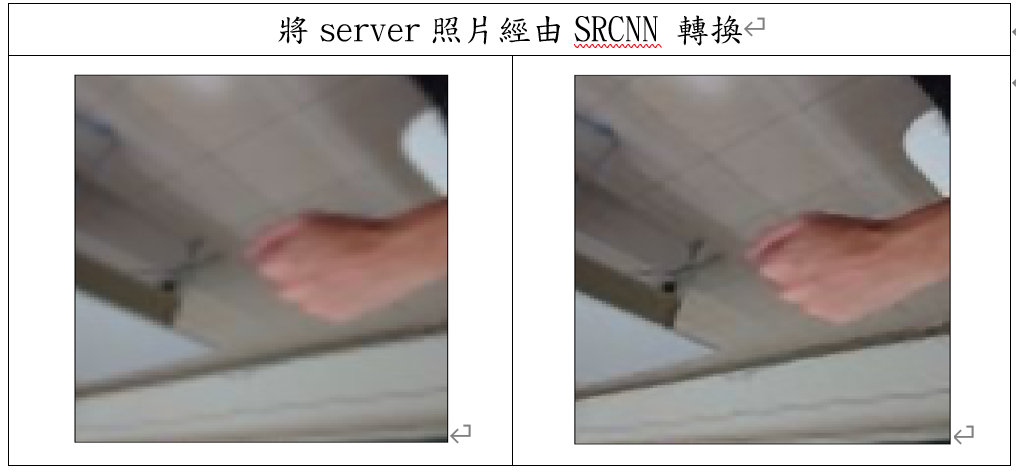
\includegraphics[width=10cm]{SRCNN_img.PNG}
    \caption{SRCNN效果圖呈現}
    \label{fig:SRCNN效果圖呈現}
\end{figure}

轉換結果評估:在未做SRCNN之前,手的輪廓並不明顯,影像顆粒度非常明顯。在做完SRCNN後,手的輪廓明顯從背景浮現,手上的陰影也更加明顯。

\subsubsection{未使用SRCNN測試結果}

\begin{figure}[H]
    \centering
    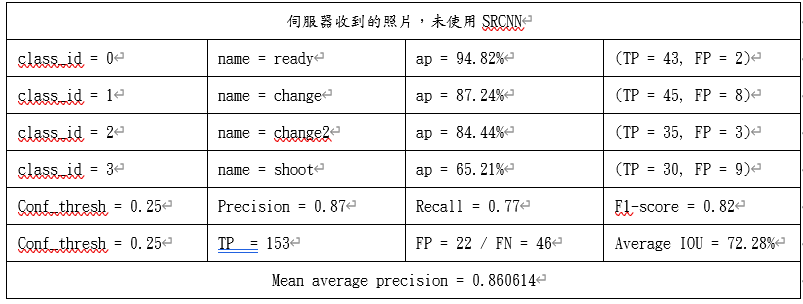
\includegraphics[width=10cm]{before_SRCNN_table.PNG}
    \caption{未使用SRCNN}
    \label{fig:未使用SRCNN}
\end{figure}

\subsubsection{使用SRCNN測試結果}

\begin{figure}[H]
    \centering
    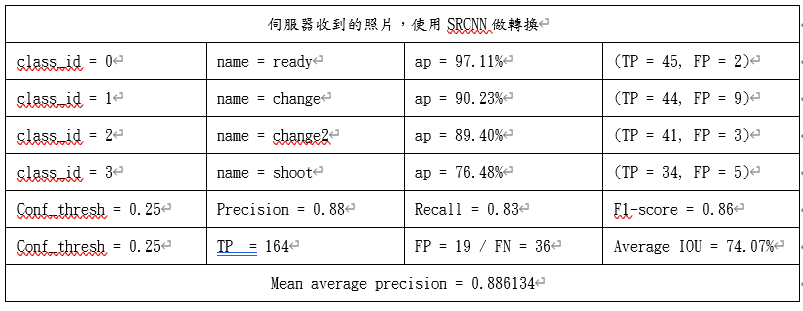
\includegraphics[width=10cm]{after_SRCNN_table.PNG}
    \caption{使用SRCNN}
    \label{fig:使用SRCNN}
\end{figure}

\begin{figure}[H]
    \centering
    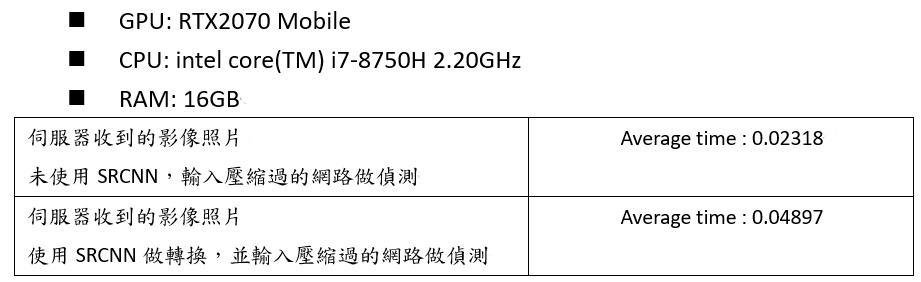
\includegraphics[width=10cm]{SRCNN_time.PNG}
    \caption{時間評估}
    \label{時間評估}
\end{figure}


評估:未做SRCNN之前,手的輪廓並不明顯,影像顆粒度非常明顯。做完SRCNN後,手的輪廓明顯從背景浮現,手上的陰影也更加明顯。使用SRCNN後mAP上升了2.5%。另外,做更深的細部分析。在最難判斷的類別id2、id3準確度皆有上升。推測可能是因為手的輪廓更明顯,從背景中凸顯出來,使手部物件辨識更加容易抓取手部位置,並更容易分類。另外,也沒有明顯的顆粒感在干擾CNN藉由filter擷取特徵的過程。
手部物件辨識:

\subsubsection{手部物件辨識網路訓練曲線圖}

\begin{figure}[H]
    \centering
    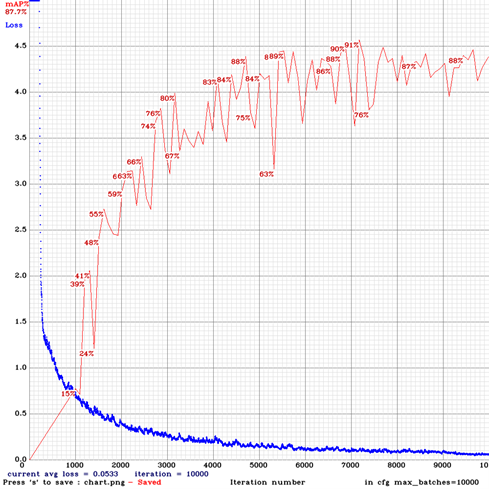
\includegraphics[width=10cm]{Darknet_Training_Curve_final.png}
    \caption{訓練曲線圖(Iteration)}
    \label{fig:訓練曲線圖(Iteration)}
\end{figure}

\begin{figure}[H]
    \centering
    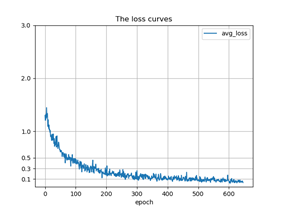
\includegraphics[width=10cm]{Darknet_Training_Curve2_final.png}
    \caption{訓練曲線圖(Epoch)}
    \label{fig:訓練曲線圖(Epoch)}
\end{figure}


觀察上方訓練結果,並沒有特別發現出現underfitting 或是 overfitting 的情形,雖然mAP以及loss在最後趨於穩定,表示其實learning rate 可以查是在做遞減,但是以整體訓練結果來看,validation data 測試所得的average mAP達到87.7%,表示訓練上收斂良好。

\subsubsection{新修改的CNN網路與原Yolo網路效能比較}

\begin{figure}[H]
    \centering
    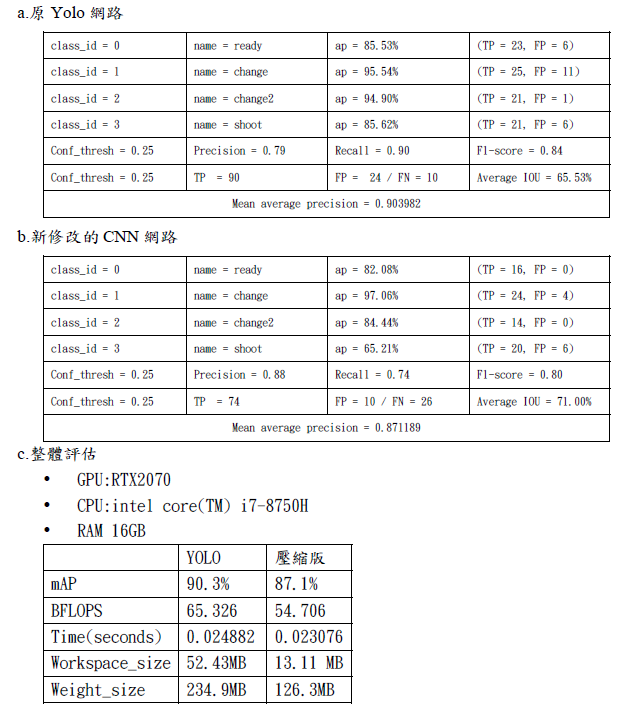
\includegraphics[width=15cm]{Darknet_Training_Table_final.PNG}
    \caption{效能比較}
    \label{fig:效能比較}
\end{figure}




\subsubsection{window設計}

\begin{itemize}
\item X軸:單位時間
\item Y軸:次數
\end{itemize}

\begin{figure}[H]
    \centering
    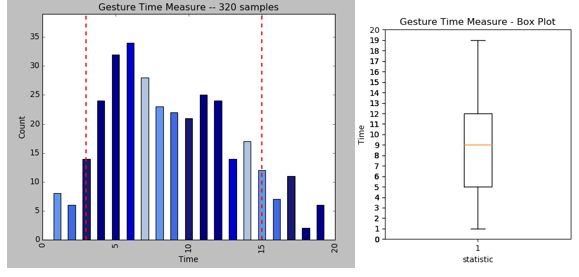
\includegraphics[width=10cm]{Windows_Size.PNG}
    \caption{window實驗}
    \label{fig:window實驗}
\end{figure}

\subsubsection{LSTM網路設計實驗}

訓練資料生成:利用手部物件辨識得到的機率分布存成檔案,再將內部行數控制在window大小。由於資料不足,所以需要做資料擴充。利用random將機率做微調以及利用平移分布的方式,達到訓練資料擴充。
訓練資料共有500筆資料,切出200筆做為測試資料,評估模型。並將訓練資料由300筆增加至30000筆。

網路設計:
\begin{itemize}
\item 輸入維度  64 14 4
\item 將hidden state通過全連接層與sigmoid後輸出類別機率
\item 輸出機率0至1,threshold = 0.5,分為兩類發射(1)與無動作(0)
\item 學習率: Learning rate = 0.0001
\item 最佳化工具: Adam Optimizer
\item 損失函數: binary cross entropy
\item 未使用dropout
\item 訓練測試資料集比例0.8
\item 訓練次數100 epoch
\end{itemize}

\begin{figure}[H]
    \centering
    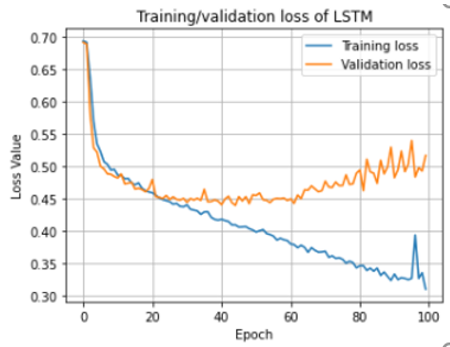
\includegraphics[width=10cm]{LSTM_Training_Curve.PNG}
    \caption{LSTM訓練曲線}
    \label{fig:LSTM訓練曲線}
\end{figure}

觀察上面Loss後,使用early stop技巧,將40 epoch 做為測試權重。
測試評估:使用真實資料100筆,各類別皆50筆,以避免資料分布不均導致評估不公正。

\begin{figure}[H]
    \centering
    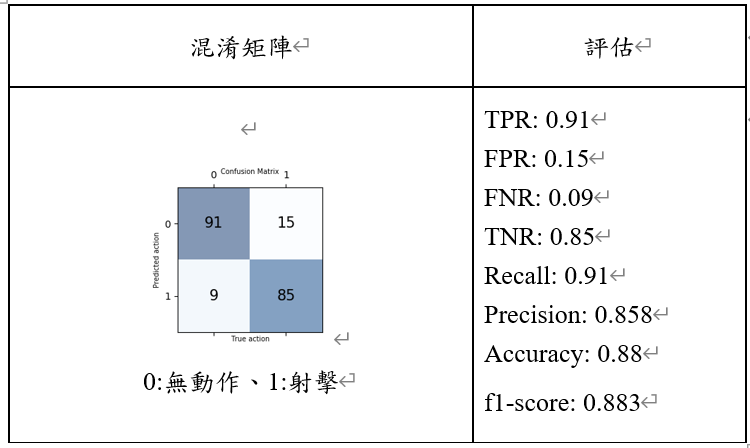
\includegraphics[width=10cm]{LSTM_Training_Table.PNG}
    \caption{手部辨識神經網路測試}
    \label{fig:手部辨識神經網路測試}
\end{figure}

分析:
由上面混淆矩陣,分類於第一類別(無動作)的正確率較高,而第二類別(射擊)的正確率相對較低。原因是,在製造第一類別(無動作)訓練資料時,可以將無動作訓練資料主要可以分為兩個類別,純粹無動作、或是有動作(但非射擊動作)。在第一部分純粹無動作是幾乎不會分類錯誤的,所以造成部份測試幾乎絕對正確。以至於第一類別(無動作)會正確率相較於第二類別(射擊)高。


\subsubsection{整體評估}
實驗方法:

使用200部影片,發射動作影片與無動作影片皆100部。給手部辨識神經網路辨識,辨識後根據該項實驗的設計來決定是否要傳送給SRCNN做高解析化,最後傳輸給LSTM網路做辨識。以LSTM網路辨識的準確度,以及整體辨識時間作為評估依據。

實驗設計:
\begin{itemize}
\item 實驗一:未優化darknet讀取影像照片方式
\item 未使用SRCNN + 未壓縮過後的手部辨識網路 + 單層LSTM輸出
\item 實驗二:優化darknet讀取影像照片方式
\item 未使用SRCNN + 未壓縮過後的手部辨識網路 + 單層LSTM輸出
\item 實驗三:優化darknet讀取影像照片方式
\item 未使用SRCNN + 壓縮過後的手部辨識網路 + 單層LSTM輸出
\item 實驗四:優化darknet讀取影像照片方式
\item 使用SRCNN + 壓縮過後的手部辨識網路 + 單層LSTM輸出
\end{itemize}

\begin{figure}[H]
    \centering
    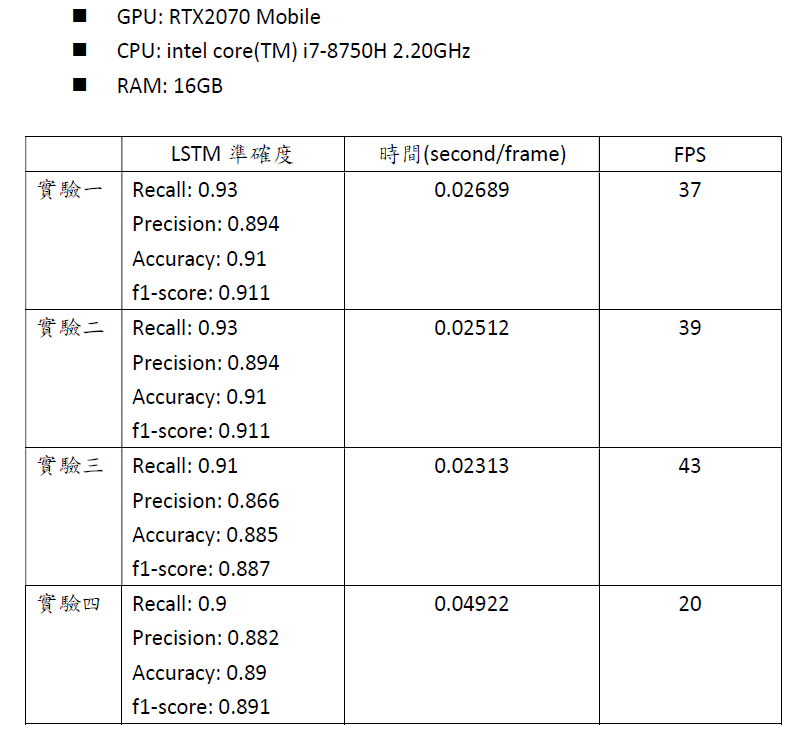
\includegraphics[width=10cm]{SUM_UP_EVAL.PNG}
    \caption{整體評估}
    \label{fig:整體評估}
\end{figure}


未壓縮優化的實驗一與加速優化的實驗三比較,FPS上升6。正確率卻只下降0.015。本專案在準確度達到一定要求下,會以縮短反應時間為主。因此選擇實驗三為本專題主要的偵測模式。
另外,對於額外使用SRCNN的實驗四來說,增加了高解析化後,雖然在(9)SRCNN實驗中顯示mAP上0.02,但是對於LSTM辨識結果並沒有太大作用,僅對於整體辨識結果正確率卻只上升0.05。而且辨識時間還增加一倍。因此往後的研究方向會以加速高解析化網路為主。

\begin{itemize}
\item 結論: 選擇實驗三作為目前專題的偵測模式。
\end{itemize}
